%!TEX root = ../document.tex
\chapter{Empirical settings and methods}
In this chapter, we will present the empirical setting and methods used in this thesis. First we will describe the empirical setting in which the data collection took place. Then we will proceed to present the methods for gathering data with a description of the technicalities of the data. Lastly, we will describe the procedures for approaching, selecting and analyzing the data.

%\section{Case Study}
%vet ikke helt hva jeg har starta her, tror jeg må lese noen oppgaver med casestudy.
%In our thesis, we have chosen gather data through a qualitative case study.  One of the most important reasons for choosing a case study was as \citet{yin2003case} states: "you want to cover contextual conditions because you believe they are relevant to the phenomenon under study". As the case was students inquiry about photosynthesis, it could not be examined without the context, the school, or more precisely the biology classroom setting where Monoplant was inserted. 

\section{Design based research}
%understand how people learn, and design ways to better ensure that learning will happen in these settings
As students from the department of informatics we have been schooled in the scandinavian model for system design where the design of software is seen as intertwined with the organizational interactions that surrounds its use \citep{bjerknes1987computers}. We are therefore used to thinking of technology within the context that it's used. \citeauthor{brown1992design}'s (\citeyear{brown1992design}) design experiments methodology was therefore well suited for the work with this thesis, as design experiments lets us take into account all the aspects of the classroom education when inserting technology into it. Or as \citet{brown1992design} defines it: "I attempt to engineer innovative educational environments and simoultaneously conduct experimental studies of those innovations".

One of \citeauthor{brown1992design}s main points is that there are several independent aspects that make up the classroom. Teacher training, curriculum, institutional aspects, etc. These parts make up a whole operating system and affect each other in complex ways. This implies that we cannot isolate certain elements of the context and analyze them in laboratory settings, as the whole is more than merely the sum of its parts \citep{brown1992design}.

%As students from department of informatics we are pragmatic in the way we approach educational research. Design experiments is therefore a good way to 

As Monoplant is designed for use in educational settings, it could not be examined without taking into account the context in which it was inserted. Design based research as a methodology lets us focus on the contextual aspects that become "relevant in the students' interactions" \citep{krange2009historical}. This means that we do not limit ourselves to merely the technical aspects of Monoplant when inserting it to the context, but take the whole into account in looking at how the technical solution provides a new context for interaction. 

%As we strongly believe that technical systems should be designed and tested in the context they are meant to be used in, it would not make sense to insert Monoplant in a non-natural environment. 

\section{Empirical setting}
The collection of data material used in this thesis took part in late autumn 2013, at a high school located in the center of Oslo. The school has a high threshold for admission, with a lower requirement of 43.5 points out of 60 in 2010 \citep{utdanningsetaten}. Thus, the students at this school are (mostly) high achievers. 

Through Intermedia, we sent out a presentational flier to different schools in Oslo (see chapter \ref{prosjektbeskrivelse} on page \pageref{prosjektbeskrivelse}). A teacher contacted us, and luckily our request coincided perfectly with a two week period dedicated to reviewing photosynthesis in his biology class. The teacher was therefore willing to test out our application instead of performing one of the experiments described in the textbook. 

The class selected was a biology class at the highest level offered at the school, biology 2, which has an extensive curriculum covering e.g., photosynthesis, enzymes and energy transmitters \citep{bios}. The class consisted of 11 girls and three boys between 17 and 18 years of age (vg3). For the main part of our data collection, all of the students were present. All of them agreed to participate in the study, but due to technical limitations and a busy time schedule, the primary data collection was  done with a small sample of the group. 


\subsection{Planning the experiments}
An initial planning and presentational meeting was with the teacher on the 21st of October. A thorough presentation and demonstration of the system was given, followed by a discussion of the functionality of the system, to see if it would spark some ideas for experiments. 

Stressing the importance of a scientific method, the teacher suggested that we could conduct two experiments. Using the different sensors in the system to control the change of one variable, while keeping the others relatively controlled. We agreed that the factor that would be easiest to control, yet yield interesting results was light intensity and light quality (wavelength). The first experiment would involve keeping the plant located in a window facing west, receiving sunlight and light from the fluorescent indoor-lighting. While we in the second experiment would relocate the plant to a light proof cabinet where it would only receive light of a known wavelength. Each of the two experiments would last one week, depending on the time needed for measurable results.

\subsection{The experiments}
The project was presented for the class during a one hour lecture on Friday 25th of October. We used the opportunity to give an in-depth explanation and demonstration of Monoplant, as well as explaining how we would collect and use the data material gathered. We then proceeded to initiate the first experiment, which went on for seven days until Friday 1st of November when the second experiment was initiated. The second experiment went on for 13 days until Wednesday 13th of November when the primary data collection session took place. During the experiments we as observers and researchers were present at four separate occasions, observing what the teacher was focusing on, and the nature of the class discussions. In addition we answered any questions they had regarding the system, and observed how it was used by the teacher and how the students interacted with it. 

\begin{figure}
\centering
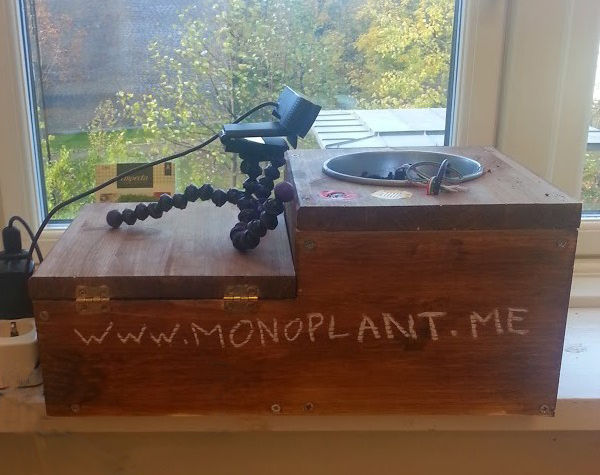
\includegraphics[width=0.8\textwidth]{img/empiricalsetting/window.jpg}
\caption{The experimental setup located in the window}
\label{fig:windowplant}
\end{figure}

\begin{figure}
\centering
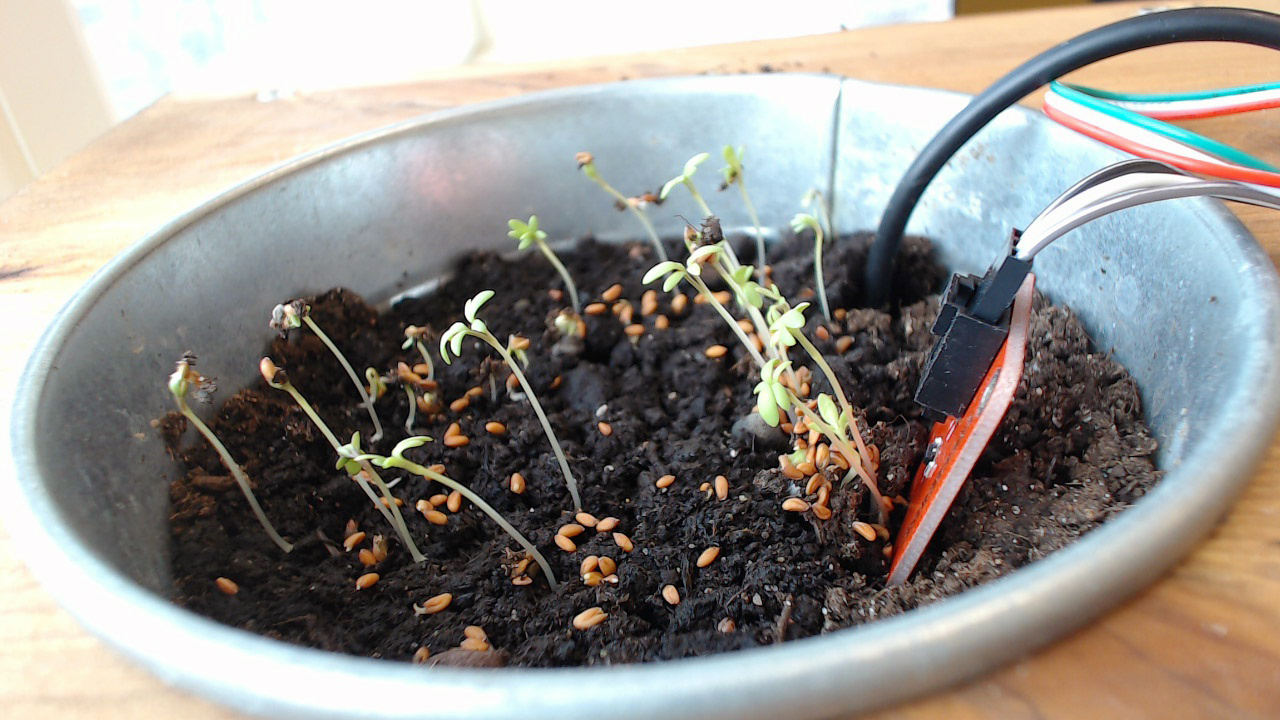
\includegraphics[width=0.8\textwidth]{img/empiricalsetting/windowsystem.jpg}
\caption{The plant receiving natural light}
\label{fig:windowsystemplant}
\end{figure}

\subsubsection*{The plant in the window}
The first experiment was conducted with a setup in the window as shown in figure~\ref{fig:windowplant}. The system was located in the front of the classroom near a door leading to an adjacent classroom, visible and in reach of everyone walking by. As figure~\ref{fig:windowsystemplant} shows, there is between 50 and 70 seeds in the pot. The plant was located in the window sill, exposed to sunlight or daylight depending on the weather, in addition to the fluorescent indoor-lighting. Due to the time of year, and lack of people using the classroom in the evening, this meant that the plant would get light in the period between 08:00 and 17:00.

It turned out that the system was draining power from a power outlet that was either connected to the indoor light or timer based, as the system went down and did not post data between 19:00 and 07:00. We also had some technical issues with the system from 25th of October to 27th of October, resulting in loss of data of the first seeds germinating.

\begin{figure}
\centering
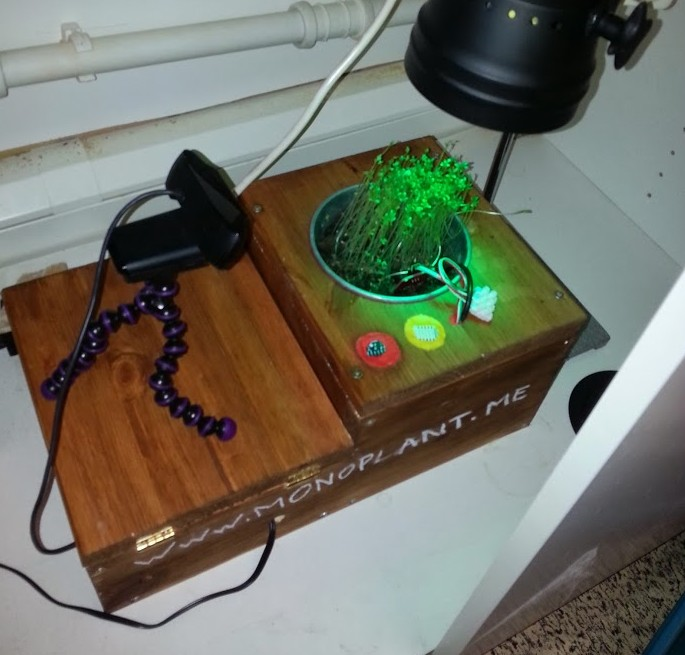
\includegraphics[width=0.8\textwidth]{img/empiricalsetting/cupboard.jpg}
\caption{The system located in the cabinet}
\label{fig:cabinetplant}
\end{figure}

\begin{figure}
\centering
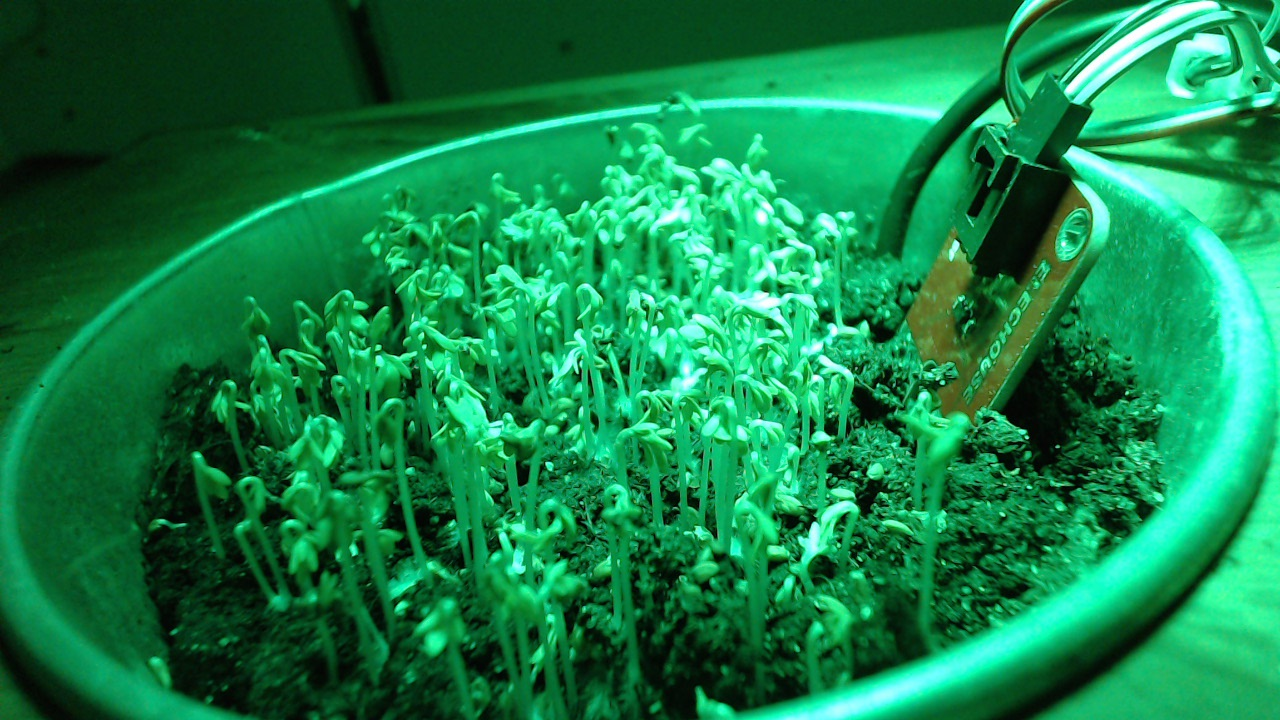
\includegraphics[width=0.8\textwidth]{img/empiricalsetting/cupboardsystem.jpg}
\caption{The plant in the cabinet, receiving green light}
\label{fig:cabinetsystemplant}
\end{figure}

\subsubsection*{The plant in the cabinet}
The second experiment was conducted with a setup in a cabinet as shown in figure~\ref{fig:cabinetplant}. The cabinet was located in a corner in the front of the classroom behind the teacher's desk, hidden and not nearly as accessible as the plant in the window. The picture in figure~\ref{fig:cabinetplant} is taken with light from the room coming in to the cabinet, hence it does not reflect the lighting conditions in the cabinet during the experiment. The cabinet door was closed and the lamp above the plant was emitting green light 24 hours a day, hence figure~\ref{fig:cabinetsystemplant} shows the lighting conditions more correctly. It is also worth noting that the pot contains around 30-40 seeds more than in the first experiment. When this experiment took place we did not have any technical issues, the system posted data continuously for the whole period.


\section{Methods}
Different methods for data collection was discussed and reviewed early on in the project. Our most influential source was the tradition for using qualitative research methods in information systems research in the design group at department of informatics. As our primary data source we chose video data with the use of multiple cameras and a screen dump. This was collected during a 45-minute session after the completion of the experiments, resulting in 3x45 minutes of video data and 45 minutes of audio data. Supplementary data from this session includes the written answers from the groups that were not filmed, and our personal notes. In the following sections the methods used will be discussed. 

\subsection{Video and audio}
It was determined early in the project that video and audio recording were to be used. The primary reason for this was the tradition at Intermedia, as video data collection has been used and thoroughly tested by a number of researchers here. This meant that we would get a lot of help from co-located researchers in what microphones to use, placement of cameras, operation of the equipment, etc. 

A total of 45 minutes of video and audio was recorded, using three separate video sources, and three microphones. One camera was placed in front of the group, able to capture facial expressions and where the students were looking. This camera had an external microphone connected that we placed on the table in front of the students, allowing us to filter out some of the noise in the classroom. The second camera was placed behind the students on their right hand side, facing the computer screen. This camera's primary function was to capture where the students were pointing and what they were doing on the laptop. The audio source of the second camera was the built-in microphone, which proved to cover most of the audio in the classroom. In addition to the video from the cameras, we recorded a screen capture from the laptop, showing exactly what the students were doing in the system. The laptop had a built-in microphone, but due to poor audio quality, this was only used when synchronizing the different videos.
\begin{figure}
\centering
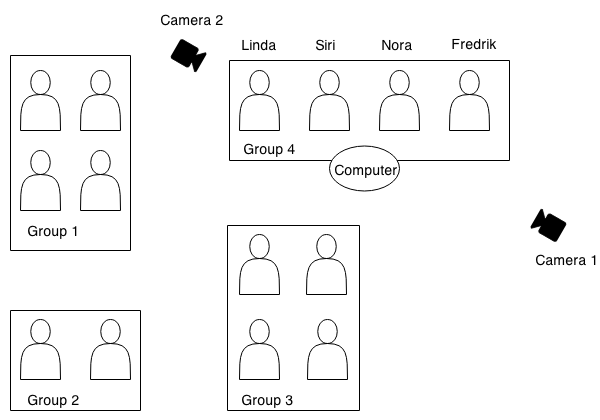
\includegraphics[width=0.8\textwidth]{img/empiricalsetting/class_diagram.png}
\caption{Camera setup}
\label{fig:camerasetup}
\end{figure}

\subsection{Passive observation}
During the experiments we were present at four separate occasions. Mostly to ensure that the system was working, assist with any technical difficulties regarding the user interface, and to ensure a smooth operation of the experiments. But we would also take notes regarding how the system was used in the lecture, if or how students showed interest in the experiments, and how the teacher was conveying information about photosynthesis in general. While these observation sessions were not thoroughly planned, and the data material never systematized, the notes from these sessions proved to be a good supplementary data source to help us structure and make sense of our primary data. We would later on also use these notes as discussion points and indexical resources when reviewing the data material. 

\subsection{Student produced material}
While we filmed the group of students selected for our main data gathering, the rest of the class was divided into groups and told to discuss and write down answers to the given assignments. These answers were handed in and digitalized by us at a later point (see chapter \ref{svaroppgaver} on page \pageref{svaroppgaver}). This became a fine supplemental data source, as it gave an insight of what answers fellow students of the class came up with in a less monitored setting. 

\subsection{Web logs}
In order to review activity on the web page (\url{http://Monoplant.me}), the Google Analytics tracking system was installed. Although we did not use this extensively, it allowed us to see if and how often the system was used, and if students were using it at home or only during classroom hours. 

\section{Analytical Procedures}
From mid November till late December 2013, we were observing, listening, transcribing and discussing the material. In this section we will describe how we approached, selected and made sense of the data once it was collected.



\subsection{Approaching the data}
\citet{derry2010conducting} speaks about two different approaches to selecting parts of a video corpus for further examination: the \emph{inductive} and the \emph{deductive} approach. Inductive approaches apply when a minimally edited video corpus is collected and investigated with broad questions in mind, but without a strong orienting theory. Deductive approaches involve identifying or creating a suitable video corpus and systematically sampling from it to examine specific research questions. \citep{derry2010conducting} To start with, we clearly fit into the inductive approach, but as many researchers have experienced: once you find something, you start looking for it. Hence our approach became more deductive as we went on with our analysis.

In order to make sense of the data gathered we looked at it in several different ways with different focuses. Below is a chronological list of the ways we approached the data. 

\begin{enumerate}
\item{Initial screening of main video corpus, locating interesting interaction}
\item{Transcription of main video corpus}
\item{Watching supplemental video material to make detailed notes on interactions with the system}
\item{Watching the main video corpus with our supervisor and discussing which events and interactions are interesting and/or can be explained by existing theory}
\item{Select parts of transcript that are of interest}
\item{Detailed transcriptions of these parts}
\item{Writing explanations for these interactions}
\item{Linking interactions to support each other}
\item{Cut excerpts that do not fit together with other excerpts}
\item{Linking chunks of interactions to related theory}
\end{enumerate}

While we still had the impressions from the data collection fresh in mind, we sat down and watched all the video material. During the screening process we tried to make a content log to get a better overview of a large corpus of data and select cue points in the video where interesting interaction took place, focusing on change in context and contradictions. This was followed by a rough transcription, using mostly audio and video from the camera facing the students. At this point we focused mostly on transcribing what was said, not paying attention to small audible details such as intonation. 

We then went on to the third step in the process, bringing in additional video material to generate thick descriptions of the interesting interactions. Using audio cues, we merged all the three video files into one, so that the screen was divided into three parts: one for the camera facing the students, one for the camera facing the screen, and one for the screen dump. This enabled us to make a more detailed transcript of the parts containing inaudible utterances.

At this point in the process we presented the transcript and screened the video along with our supervisor, marking the points in the video that we deemed most interesting. In the discussion afterwards a list of themes or grouping categories was selected, which would be subject to further analysis. A selection of excerpts from the transcripts was then picked out for further analysis where we kept focus on intonation, gestures, etc. to provide a thorough description of the events unfolding. 

As shown in the list, our approach was quite open to begin with, scanning the complete video corpus for what we found interesting. Once we began to find parts that interested us, we started to look for similar events and contradicting events. With help from our supervisor we found theoretical concepts we could link to our material, which again gave us an incentive to look for specific types of material.

\subsection{Interaction analysis}
%Crang & cook: Video recordings can be criticized by pointing out that it is the researcher that selects the frame and focus. Hence the data can become biased. However, by trying to frame interaction generically, and providing a video, getting other people to double check coding and transcription.
The analytical procedure employed within this thesis is \emph{interaction analysis} \citep{jordan1995interaction}, which emerged from fields such as ethnography, sociolinguistics, ethnomethodology, conversation analysis, and sociocultural theories. \citeauthor{jordan1995interaction} describes it as follows:

\begin{quote}
An interdisciplinary method for the empirical investigation of the interaction of human
beings with each other and with objects in their environment. It investigates human
activities such as talk, nonverbal interaction, and the use of artifacts and technologies,
identifying routine practices and problems and the resources for their solution \citep[p39]{jordan1995interaction}
\end{quote}

For Interaction analysis to become a reality video and audio recording technology has been a vital resource. The combination of recording talk as well as nonverbal interaction and the ability to replay a sequence as many times as necessary gives us the possibility to analyze more thoroughly. Combining this micro-level data of interaction with ethnographic data gives us a means of analyzing how the interaction is part of the situated context and institutional practices. \citep{furberg2009scientific}. 

\subsection{Systemic vs. dialogic}
\citet{arnseth2006approaching} introduces a distinction between two approaches to CSCL research: \emph{systemic} and \emph{dialogic}. A main feature of studies characterized to be using a \emph{systemic approach} is that they generate models of how features of the technological system reviewed affects reasoning, collaboration, structures of discourse etc. The analytical focus is on describing the systematic relations between forms of social interaction, and specific types of support or other contextual factors on the one hand, and qualities of outcome on the other. \citep{arnseth2006approaching} In other words, \emph{systemic} studies tend to measure how much a specific feature or configuration in a CSCL-tool affects learning outcomes in terms of "measurable" or "quantifiable" variables. The result of this analytical practice is often a formulation of a model or reformulation of an existing model, which may state that a CSCL application together with a certain practice, are likely to produce a positive learning outcome.

\citeauthor*{arnseth2006approaching} argue that there has been little interest in the emergent characteristics of actions that take place when CSCL-tools are introduced in schools. As they write: \emph{"we need to examine more closely how the meaning and functions of CSCL applications are actually constituted in practice."} \citep[p. 181]{arnseth2006approaching}. Hence they introduce the \emph{dialogic} approach, where CSCL applications are not treated as a variable with features and configurations that in relation to other variables i.e., learning outcome can be determined statistically. Instead, the analytical concern  of the \emph{dialogic} approach is how computer applications provide a new context for social interaction.

%\sout{ By observing the class during our visits to the school during the experiments, and by reading the textbook chapter on photosynthesis, we gathered ethnographic data on how the class worked together and what they were expected to know about photosynthesis. }

%\sout{Even though we have done a case study in a real educational setting, considering these ethnographic data is important if we are to keep a dialogic perspective.}


%\sout{At point 8 in the list, we had found over 20 excerpts that we wanted to present and discuss. By categorizing these into four themes: \emph{Hypothesis generation and testing}, \emph{Misconception}, \emph{Conceptualization} and \emph{Linking between representations}, we were able to find the best excerpts to represent the themes. Hence we ended up with 11 excerpts, which will be presented in the following chapter.}

\section{Research quality}
In this section we will briefly address the quality of our research based on \emph{credibility}, \emph{transferability}. \emph{dependability}, and \emph{confirmability} as presented by \citet{baxter1997evaluating}. We will also discuss the ethics, strengths and weaknesses. 

%credibility
\subsection{Credibility}
In qualitative research, credibility is related to the authenticity of the account, and defined as the: \begin{quote}degree to which a description of human experience is such that those having the experience would recognize it immediately and those outside the experience can understand it \citetext{\citealp{lincoln1985naturalistic}, referenced in \citealp{baxter1997evaluating}}\end{quote}

This implies that there is not one true objective reality as in the positivist paradigm, but rather multiple realities constructed by ourselves. The credibility is therefore concerned with the relation between the experiences of the participants and the concepts we use to recreate and simplify them through interpretation \citep{baxter1997evaluating}.

When we selected our research subjects, we employed the strategy of "purpousful sampling" \citep{baxter1997evaluating}. Together with the teacher we found a selection of students that were able to express their thoughts and discuss freely. They also seemed relatively unaffected by our presence and the presence of cameras. Prior to the selection we also made sure that none of the students would feel uncomfortable being filmed. This helped us get an information rich case with many different experiences to answer our research questions. 

We were present at numerous occasions during our contact with the high school. This helped us get a better picture of the dynamics of the biology class. So while our main corpus of data is a one hour video, our analysis is informed by a larger picture of the situation. During these visits we made observation notes, which are also included in our data material. This is a strategy called triangulation of methods \citep{baxter1997evaluating}, which suggests that different methods can mutually support one another. 

During data collection we were at all times two researchers observing the same situations. This helped us create "thicker" \citep{geertz1973interpretation} accounts of the situations by discussing the content among ourselves. We also included our supervisor in screening of the video data to get more perspectives on the same data material. Variations in interpretations of the events unfolding was also discussed.

All of these strategies combined helps to ensure the accuracy of the experiences described in our data material. 

\subsection{Transferability}
Transferability refers to the degree to which the findings in one study can fit in other contexts \citep{baxter1997evaluating}. In qualitative research, results can naturally not be replicated as in a science experiment, however we can judge if findings in our study are applicable to similar educational settings. Meanings are often shared by many individuals, and it is possible that the experiences described in our study will fit to similar groups. 
While we will make no claim about the transferability of our study, we have tried to provide as thick descriptions as possible. We have also included our data material in the appendices so the readers themselves can determine the degree of transferability of our results. 

\subsection{Dependability}
Dependability is defined by \citet{baxter1997evaluating} as "the degree to which it is possible to deal with instability/idiosyncrasy and desgin-induced change". This refers to the consistency of the qualitative study, so that the "same constructs may be matched with the same phenomena over space and time" \citep{baxter1997evaluating}. 

To deal with the threats against dependability we have made use of mechanically recorded data, which has been transcribed verbatim by two researchers. We have consistently used a standardized transcript notation. Low inference descriptors has been used when possible, and while dealing with inaudible data, we have tried to provide thick descriptions in our data material. Our supervisor has also functioned as an auditor and "ensured that appropriate decisions were are made along the way" \citep{baxter1997evaluating}
%confirmability

\subsection{Confirmability}
\citet{lincoln1985naturalistic} defines confirmability as "the degree to which findings are determined by the respondents and conditions of the inquiry and not by the biases, motivations, interests or perspectives of the inquirer". During our research we have made a series of choices that have been guided by our interests, prior knowledge, experience, and perspectives. Throughout this thesis we have tried to provide a rationale for the choices made. We have also included all of our raw material in the appendices, the data selection in the data chapter, and our analysis and rationale for analysis. In doing so, we hope to have given the reader the instruments needed to assess the confirmability of our research.  

Altogether, these strategies have increased the quality of our research. This being said, we are well aware that further steps could have been taken. We could for instance have sent our analysis of the data to the participants to see if they agreed on our interpretations of the events. We could also have immersed ourselves deeper in the situation and collected more data material from a larger selection of students. This has not been done due to time limitations. 

\subsection{Ethics}
Prior to the data collection, an application was sent to NSD (Norwegian Social Science Data Services) requesting permission to film the students. The application was approved with only minor changes to how the material was to be treated after completion. In addition all the students taking the class were given an consent form stating that participation was voluntary, and all material would be kept anonymous (see chapter \ref{samtykkeskjema} on page \pageref{samtykkeskjema}). 

Throughout this thesis, and in the transcripts of video data, all the students' names have been replaced by pseudonyms and the name of the school is never mentioned. The data material containing identifying information of the students has been and will be stored securely on a separate hard drive at Intermedia, and will be deleted  upon termination of the project. 

During our time at the school we were always open about our role as researchers, and explained on several occasions how the data was going to be used. 

